\documentclass[fleqn,11pt,aspectratio=43]{beamer}
\usepackage[utf8x]{inputenc}
\usepackage[T1]{fontenc}
\usepackage[ngerman]{babel}
\usepackage{stmaryrd}
\usepackage{amsfonts}
\usepackage{amssymb}
\usepackage{amsmath}
\usepackage{microtype}

\usepackage{listings}
\usepackage{color}
\usepackage{pxfonts}

\definecolor{mygreen}{RGB}{51,141,120}
\definecolor{myblue}{RGB}{0,128,180}
\definecolor{myviolet}{RGB}{118,0,118}

\lstset{ %
  language=Haskell,
  backgroundcolor=\color{white},         % choose the background color
  basicstyle=\ttfamily\footnotesize,     % size of fonts used for the code
  numbers=none,
  breaklines=true,                       % automatic line breaking only at whitespace
  captionpos=b,                          % sets the caption-position to bottom
  commentstyle=\color{mygreen},    % comment style
  escapeinside={\%*}{*)},                % if you want to add LaTeX within your code
  keywordstyle=\color{myblue}\bfseries, % keyword style
  stringstyle=\color{myviolet},    % string literal style
  frame=single,
  tabsize=2
}
\usepackage{tikz}
\usetikzlibrary{
  arrows,
  shapes.misc,
  shapes.arrows,
  chains,
  matrix,
  positioning,
  scopes,
  decorations.pathmorphing,
  shadows,
  backgrounds
}


\usetheme[%
  %cmyk,%<cmyk/rgbprint>,          Auswahl des Farbmodells
  orange,%<blue/orange/green/violet> Auswahl des Sekundärfarbklangs
  %dark,%<light,medium>        Auswahl der Helligkeit
  %colorhead,%    Farbig hinterlegte Kopfleiste
  %colorfoot,%    Farbig hinterlegt Fußleiste auf Titelseite
  %colorblocks,%   Blöcke Farbig hinterlegen
  %nopagenum,%    Keine Seitennumer in Fußzeile
  %nodate,%       Kein Datum in Fußleiste
  %tocinheader,%   Inhaltsverzeichnis in Kopfleiste
  %tinytocinheader,% kleines Kopfleisten-Inhaltsverzeichnis
  %widetoc,%      breites Kopfleisten-Inhaltsverzeichnis
  %narrowtoc,%    schmales Kopfleisten-Inhaltsverzeichnis
  %nosubsectionsinheader,%  Keine subsections im Kopfleisten-Inhaltsverzeichnis
  %nologoinfoot,% Kein Logo im Fußbereich darstellen
  ]{tubs}

\titlegraphic[scaled]{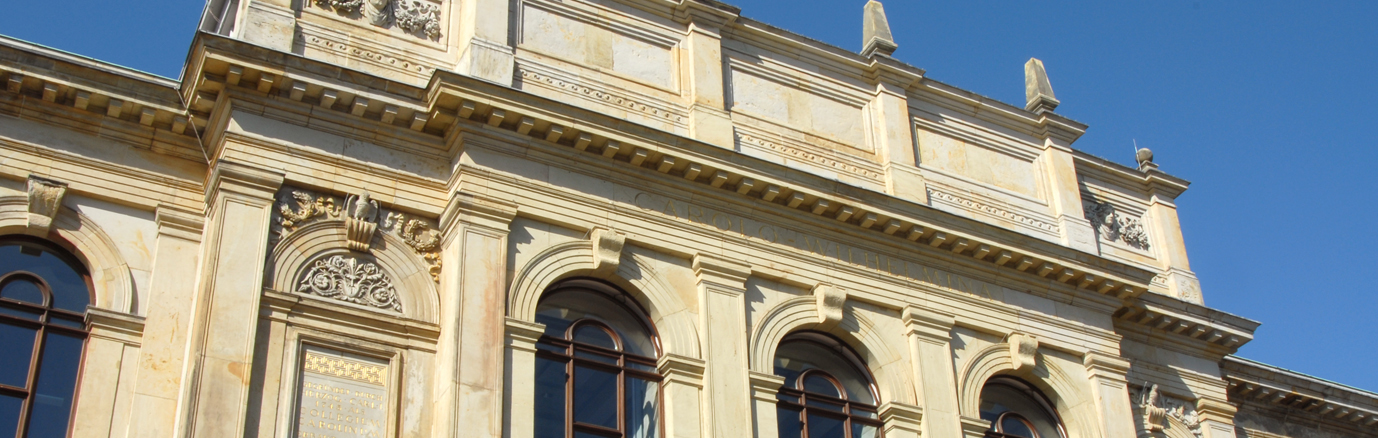
\includegraphics{img/titlepicture.jpg}}
\logo{
\includegraphics{img/logo_mit_text.pdf}}

\AtBeginSection[]{
  \begin{frame}[noframenumbering] 
  		\scriptsize
  		\frametitle{Überblick}  
  		\tableofcontents[currentsection, hideallsubsections]
  \end{frame}
}

\AtBeginSubsection[]{
  \begin{frame}[noframenumbering]
    	\scriptsize 
  		\frametitle{\insertsectionhead - \insertsubsectionhead} 
  		\tableofcontents[ 
  			currentsubsection, 
  		    sectionstyle=show/hide, 
  		   	subsectionstyle=show/shaded/hide] 
  \end{frame}
}


\title{Programmieren für Fortgeschrittene - \\eine Einführung in Haskell}

\author[Stephan Mielke]{\emph{Stephan Mielke}}
\institute[TU Braunschweig, IPS]{Technische Universität Braunschweig, IPS}

\begin{document}

\subtitle{Teil zwei - etwas mehr} 
\date{01.12.2014}

\begin{frame}[plain, noframenumbering]
\titlepage
\end{frame}

\begin{frame}[noframenumbering]
  \scriptsize
  %\frametitle{\insertsectionhead}  
  \frametitle{Überblick}  
  %\begin{block}{\vspace*{-2ex}}
    \tableofcontents[currentsection,sectionstyle=show, hideallsubsections]
  %end{block} 
\end{frame}


\section{Gültigkeitsbereiche~}
\subsection{Block}
%\begin{frame}
%\frametitle{Block}
%\begin{block}{\vspace*{-3ex}}
%\begin{itemize}
%  \item Definitionen im Block sind immer nur eine Stufe höher sichtbar (hier sind nicht let-in und where gemeint)
%  \item Im Block ist alles Äußere sichtbar
%\end{itemize}
%\end{block}
%\end{frame}

\begin{frame}
\frametitle{Block - Einrückungen}
\begin{block}{\vspace*{-3ex}}
\begin{itemize}
  \item In Haskell spielt das Layout des Quellcodes eine Rolle!
  \item Blöcke werden durch gleiche Einrückungstiefe kenntlich gemacht
  \item Einzelne Deklarationen werden durch Zeilenumbrüche getrennt
  \item Beginnt eine neue Zeile gegenüber dem aktuellen Block 
  \begin{itemize}
    \item \dots Rechts eingerückt: aktuelle Zeile wird fortgesetzt
    \item \dots Links eingerückt: aktueller Block wird beendet
    \item \dots Direkt an seinem "`linken Rand darunter"', so wird der Block fortgesetzt bzw. eine neue Deklaration eingeleitet 
  \end{itemize}
\end{itemize}
\end{block}
\end{frame}

%\begin{frame}[fragile]
%\frametitle{Block} 
%\begin{lstlisting}
%outer a b =
%  let inner c = a + b + c
%  in inner 1
%\end{lstlisting}
%\end{frame}
\subsection{Module}
\begin{frame}
\frametitle{Module}
\begin{block}{\vspace*{-3ex}}
\begin{itemize}
  \item Das Programm kann in Module aufgeteilt werden
  \item Der Standard-Modulname ist Main
  \item Module müssen mit einem Großbuchstaben beginnen
  \item Vorteile: 
    \begin{itemize}
      \item Vereinfachung des Programmdesigns, Strukturierung
      \item Einfachere Isolation von Fehlern
      \item Einfaches Ändern von Teilkomponenten ohne Einfluss auf andere Teile
      \item Wiederverwendung von Code
    \end{itemize}
\end{itemize}
\end{block}
\end{frame}

\begin{frame}[fragile]
\frametitle{Module}
\begin{block}{\vspace*{-3ex}}
\begin{center}
\scalebox{1}{\begin{tikzpicture}[
      nonterminal/.style={
         rectangle,
         minimum size=5.0mm,
         very thick,
         draw=blue!50!black!50,
         top color=white,
         bottom color=blue!50!black!20,
         font=\itshape\scriptsize,
         %text height=1.5ex,
         %text depth=.25ex
      },
      terminal/.style={
         rounded rectangle,
         minimum size=5.0mm,
         very thick,draw=black!50,
         top color=white,bottom color=black!20,
         font=\ttfamily\scriptsize,
         %text height=1.5ex,
         %text depth=.25ex
      },
      skip loop/.style={
         to path={-- ++(0,#1) -| (\tikztotarget)}
      },
      point/.style={coordinate},>=stealth',thick,draw=black!50,
      tip/.style={->,shorten >=0.007pt},every join/.style={rounded corners},
      hv path/.style={to path={-| (\tikztotarget)}},
      vh path/.style={to path={|- (\tikztotarget)}},
      %text height=1.5ex,text depth=.25ex
    ]
    \matrix[column sep=5.0mm, row sep=3.0mm] {
\node (n11) [circle, draw, inner sep=0pt, minimum size=0.75ex] {}; & \node (n12) [terminal] {module}; & \node (n13) [nonterminal] {Name}; & \node (n14) [terminal] {where}; & \node (n15) [terminal] {LF}; & \node (n16) [point] {};\\
 &  &  &  &  & \\
\node (n31) [point] {}; & \node (n32) [nonterminal] {Funktionensdefinitionen}; & \node (n33) [circle, draw, inner sep=0pt, minimum size=0.75ex] {}; &  &  & \\
    };
  { [start chain]
       \chainin (n11);
       \chainin (n12)    [join=by tip];
  }
  { [start chain]
       \chainin (n12);
       \chainin (n13)    [join=by tip];
  }
  { [start chain]
       \chainin (n13);
       \chainin (n14)    [join=by tip];
  }
  { [start chain]
       \chainin (n14);
       \chainin (n15)    [join=by tip];
  }
  { [start chain]
       \chainin (n15);
       \chainin (n16)    [join=by tip];
  }
  { [start chain]
       \chainin (n31);
       \chainin (n32)    [join=by tip];
  }
  { [start chain]
       \chainin (n32);
       \chainin (n33)    [join=by tip];
  }
\end{tikzpicture}
}
\end{center}
\end{block} 
\end{frame}

\begin{frame}[fragile]
\frametitle{Module} 
\begin{lstlisting}
module Wurf where
weite :: Double -> Double -> Double
weite v0 phi = ((square v0) / 9.81) * sin (2 * phi)
square :: Double -> Double
square x = x * x
\end{lstlisting}
\begin{lstlisting}
module Foo where
import Wurf
foo ... = ... (weite v w) ...
bar ... = ... (square a) ...
\end{lstlisting}
\end{frame}

\begin{frame}
\frametitle{Module - Interfaces}
\only<1>{
\begin{block}{Import}
\begin{center}
\scalebox{1}{\begin{tikzpicture}[
      nonterminal/.style={
         rectangle,
         minimum size=5.0mm,
         very thick,
         draw=blue!50!black!50,
         top color=white,
         bottom color=blue!50!black!20,
         font=\itshape\scriptsize,
         %text height=1.5ex,
         %text depth=.25ex
      },
      terminal/.style={
         rounded rectangle,
         minimum size=5.0mm,
         very thick,draw=black!50,
         top color=white,bottom color=black!20,
         font=\ttfamily\scriptsize,
         %text height=1.5ex,
         %text depth=.25ex
      },
      skip loop/.style={
         to path={-- ++(0,#1) -| (\tikztotarget)}
      },
      point/.style={coordinate},>=stealth',thick,draw=black!50,
      tip/.style={->,shorten >=0.007pt},every join/.style={rounded corners},
      hv path/.style={to path={-| (\tikztotarget)}},
      vh path/.style={to path={|- (\tikztotarget)}},
      %text height=1.5ex,text depth=.25ex
    ]
    \matrix[column sep=5.0mm, row sep=3.0mm] {
\node (n11) [circle, draw, inner sep=0pt, minimum size=0.75ex] {}; & \node (n12) [terminal] {module}; & \node (n13) [nonterminal] {Name}; & \node (n14) [terminal] {where}; & \node (n15) [terminal] {LF}; & \node (n16) [point] {}; &  & \\
 &  &  &  &  &  &  & \\
 &  &  &  & \node (n35) [nonterminal] {Name}; & \node (n36) [terminal] {,}; &  & \\
\node (n41) [point] {}; & \node (n42) [terminal] {import}; & \node (n43) [nonterminal] {Name}; & \node (n44) [point] {}; &  &  & \node (n47) [point] {}; & \node (n48) [point] {};\\
 &  &  &  &  &  &  & \\
\node (n61) [point] {}; & \node (n62) [nonterminal] {Funktionendefinitionen}; & \node (n63) [circle, draw, inner sep=0pt, minimum size=0.75ex] {}; &  &  &  &  & \\
    };
  { [start chain]
       \chainin (n11);
       \chainin (n12)    [join=by tip];
  }
  { [start chain]
       \chainin (n12);
       \chainin (n13)    [join=by tip];
  }
  { [start chain]
       \chainin (n13);
       \chainin (n14)    [join=by tip];
  }
  { [start chain]
       \chainin (n14);
       \chainin (n15)    [join=by tip];
  }
  { [start chain]
       \chainin (n15);
       \chainin (n16)    [join=by tip];
  }
  { [start chain]
       \chainin (n41);
       \chainin (n42)    [join=by tip];
  }
  { [start chain]
       \chainin (n42);
       \chainin (n43)    [join=by tip];
  }
  { [start chain]
       \chainin (n43);
       \chainin (n44)    [join];
  }
  { [start chain]
       \chainin (n44);
       \chainin (n47)    [join];
  }
  { [start chain]
       \chainin (n36);
       \chainin (n35)    [join=by tip];
  }
  { [start chain]
       \chainin (n47);
       \chainin (n36)    [join=by {vh path,tip}];
  }
  { [start chain]
       \chainin (n35);
       \chainin (n44)    [join=by {hv path,tip}];
  }
  { [start chain]
       \chainin (n47);
       \chainin (n48)    [join=by tip];
  }
  { [start chain]
       \chainin (n61);
       \chainin (n62)    [join=by tip];
  }
  { [start chain]
       \chainin (n62);
       \chainin (n63)    [join=by tip];
  }
\end{tikzpicture}
}
\end{center}
\end{block}
}
\only<2>{
\begin{block}{Selektiver Import}
\begin{center}
\scalebox{0.7}{\begin{tikzpicture}[
      nonterminal/.style={
         rectangle,
         minimum size=5.0mm,
         very thick,
         draw=blue!50!black!50,
         top color=white,
         bottom color=blue!50!black!20,
         font=\itshape\scriptsize,
         %text height=1.5ex,
         %text depth=.25ex
      },
      terminal/.style={
         rounded rectangle,
         minimum size=5.0mm,
         very thick,draw=black!50,
         top color=white,bottom color=black!20,
         font=\ttfamily\scriptsize,
         %text height=1.5ex,
         %text depth=.25ex
      },
      skip loop/.style={
         to path={-- ++(0,#1) -| (\tikztotarget)}
      },
      point/.style={coordinate},>=stealth',thick,draw=black!50,
      tip/.style={->,shorten >=0.007pt},every join/.style={rounded corners},
      hv path/.style={to path={-| (\tikztotarget)}},
      vh path/.style={to path={|- (\tikztotarget)}},
      %text height=1.5ex,text depth=.25ex
    ]
    \matrix[column sep=5.0mm, row sep=3.0mm] {
\node (n11) [circle, draw, inner sep=0pt, minimum size=0.75ex] {}; & \node (n12) [terminal] {module}; & \node (n13) [nonterminal] {Name}; & \node (n14) [terminal] {where}; & \node (n15) [terminal] {LF}; & \node (n16) [point] {}; &  &  &  &  &  &  & \\
 &  &  &  &  &  &  &  &  &  &  &  & \\
 &  &  &  &  &  & \node (n37) [point] {}; &  &  &  &  &  & \\
 &  &  &  &  &  & \node (n47) [point] {}; &  &  &  &  &  & \\
\node (n51) [point] {}; & \node (n52) [terminal] {import}; & \node (n53) [point] {}; & \node (n54) [nonterminal] {Name}; & \node (n55) [point] {}; & \node (n56) [terminal] {(}; & \node (n57) [nonterminal] {Funktion}; & \node (n58) [terminal] {,}; & \node (n59) [terminal] {)}; & \node (n510) [point] {}; & \node (n511) [terminal] {,}; & \node (n512) [point] {}; & \node (n513) [point] {};\\
 &  &  &  &  &  &  &  &  &  &  &  & \\
\node (n71) [point] {}; & \node (n72) [nonterminal] {Funktionendefinitionen}; & \node (n73) [circle, draw, inner sep=0pt, minimum size=0.75ex] {}; &  &  &  &  &  &  &  &  &  & \\
    };
  { [start chain]
       \chainin (n11);
       \chainin (n12)    [join=by tip];
  }
  { [start chain]
       \chainin (n12);
       \chainin (n13)    [join=by tip];
  }
  { [start chain]
       \chainin (n13);
       \chainin (n14)    [join=by tip];
  }
  { [start chain]
       \chainin (n14);
       \chainin (n15)    [join=by tip];
  }
  { [start chain]
       \chainin (n15);
       \chainin (n16)    [join=by tip];
  }
  { [start chain]
       \chainin (n51);
       \chainin (n52)    [join=by tip];
  }
  { [start chain]
       \chainin (n52);
       \chainin (n53)    [join];
  }
  { [start chain]
       \chainin (n53);
       \chainin (n54)    [join=by tip];
  }
  { [start chain]
       \chainin (n54);
       \chainin (n55)    [join];
  }
  { [start chain]
       \chainin (n55);
       \chainin (n56)    [join=by tip];
  }
  { [start chain]
       \chainin (n56);
       \chainin (n57)    [join=by tip];
  }
  { [start chain]
       \chainin (n57);
       \chainin (n58)    [join=by tip];
  }
  { [start chain]
       \chainin (n58);
       \chainin (n59)    [join=by tip];
  }
  { [start chain]
       \chainin (n59);
       \chainin (n510)    [join];
  }
  { [start chain]
       \chainin (n510);
       \chainin (n511)    [join=by tip];
  }
  { [start chain]
       \chainin (n511);
       \chainin (n512)    [join];
  }
  { [start chain]
       \chainin (n512);
       \chainin (n513)    [join=by tip];
  }
  { [start chain]
       \chainin (n71);
       \chainin (n72)    [join=by tip];
  }
  { [start chain]
       \chainin (n72);
       \chainin (n73)    [join=by tip];
  }
  { [start chain]
       \chainin (n510);
       \chainin (n47)    [join=by vh path];
       \chainin (n55)    [join=by {hv path,tip}];
  }
  { [start chain]
       \chainin (n512);
       \chainin (n37)    [join=by vh path];
       \chainin (n53)    [join=by {hv path,tip}];
  }
\end{tikzpicture}
}
\end{center}
Am Ende steht natürlich kein Komma
\end{block}
}
\only<3>{
\begin{block}{Negativ selektiver Import}
\begin{center}
\scalebox{0.7}{\begin{tikzpicture}[
      nonterminal/.style={
         rectangle,
         minimum size=5.0mm,
         very thick,
         draw=blue!50!black!50,
         top color=white,
         bottom color=blue!50!black!20,
         font=\itshape\scriptsize,
         %text height=1.5ex,
         %text depth=.25ex
      },
      terminal/.style={
         rounded rectangle,
         minimum size=5.0mm,
         very thick,draw=black!50,
         top color=white,bottom color=black!20,
         font=\ttfamily\scriptsize,
         %text height=1.5ex,
         %text depth=.25ex
      },
      skip loop/.style={
         to path={-- ++(0,#1) -| (\tikztotarget)}
      },
      point/.style={coordinate},>=stealth',thick,draw=black!50,
      tip/.style={->,shorten >=0.007pt},every join/.style={rounded corners},
      hv path/.style={to path={-| (\tikztotarget)}},
      vh path/.style={to path={|- (\tikztotarget)}},
      %text height=1.5ex,text depth=.25ex
    ]
    \matrix[column sep=5.0mm, row sep=3.0mm] {
\node (n11) [circle, draw, inner sep=0pt, minimum size=0.75ex] {}; & \node (n12) [terminal] {module}; & \node (n13) [nonterminal] {Name}; & \node (n14) [terminal] {where}; & \node (n15) [terminal] {LF}; & \node (n16) [point] {}; &  &  &  &  &  &  &  & \\
 &  &  &  &  &  &  &  &  &  &  &  &  & \\
 &  &  &  &  &  &  & \node (n38) [point] {}; &  &  &  &  &  & \\
 &  &  &  &  &  &  & \node (n48) [point] {}; &  &  &  &  &  & \\
\node (n51) [point] {}; & \node (n52) [terminal] {import}; & \node (n53) [point] {}; & \node (n54) [nonterminal] {Name}; & \node (n55) [terminal] {hiding}; & \node (n56) [point] {}; & \node (n57) [terminal] {(}; & \node (n58) [nonterminal] {Funktion}; & \node (n59) [terminal] {,}; & \node (n510) [terminal] {)}; & \node (n511) [point] {}; & \node (n512) [terminal] {,}; & \node (n513) [point] {}; & \node (n514) [point] {};\\
 &  &  &  &  &  &  &  &  &  &  &  &  & \\
\node (n71) [point] {}; & \node (n72) [nonterminal] {Funktionendefinitionen}; & \node (n73) [circle, draw, inner sep=0pt, minimum size=0.75ex] {}; &  &  &  &  &  &  &  &  &  &  & \\
    };
  { [start chain]
       \chainin (n11);
       \chainin (n12)    [join=by tip];
  }
  { [start chain]
       \chainin (n12);
       \chainin (n13)    [join=by tip];
  }
  { [start chain]
       \chainin (n13);
       \chainin (n14)    [join=by tip];
  }
  { [start chain]
       \chainin (n14);
       \chainin (n15)    [join=by tip];
  }
  { [start chain]
       \chainin (n15);
       \chainin (n16)    [join=by tip];
  }
  { [start chain]
       \chainin (n51);
       \chainin (n52)    [join=by tip];
  }
  { [start chain]
       \chainin (n52);
       \chainin (n53)    [join];
  }
  { [start chain]
       \chainin (n53);
       \chainin (n54)    [join=by tip];
  }
  { [start chain]
       \chainin (n54);
       \chainin (n55)    [join=by tip];
  }
  { [start chain]
       \chainin (n55);
       \chainin (n56)    [join];
  }
  { [start chain]
       \chainin (n56);
       \chainin (n57)    [join=by tip];
  }
  { [start chain]
       \chainin (n57);
       \chainin (n58)    [join=by tip];
  }
  { [start chain]
       \chainin (n58);
       \chainin (n59)    [join=by tip];
  }
  { [start chain]
       \chainin (n59);
       \chainin (n510)    [join=by tip];
  }
  { [start chain]
       \chainin (n510);
       \chainin (n511)    [join];
  }
  { [start chain]
       \chainin (n511);
       \chainin (n512)    [join=by tip];
  }
  { [start chain]
       \chainin (n512);
       \chainin (n513)    [join];
  }
  { [start chain]
       \chainin (n513);
       \chainin (n514)    [join=by tip];
  }
  { [start chain]
       \chainin (n71);
       \chainin (n72)    [join=by tip];
  }
  { [start chain]
       \chainin (n72);
       \chainin (n73)    [join=by tip];
  }
  { [start chain]
       \chainin (n511);
       \chainin (n48)    [join=by vh path];
       \chainin (n56)    [join=by {hv path,tip}];
  }
  { [start chain]
       \chainin (n513);
       \chainin (n38)    [join=by vh path];
       \chainin (n53)    [join=by {hv path,tip}];
  }
\end{tikzpicture}
}
\end{center}
Am Ende steht natürlich kein Komma
\end{block}
}
\end{frame}

\begin{frame}[fragile]
\frametitle{Module - Interfaces} 
\begin{lstlisting}
module Wurf where
weite :: Double -> Double -> Double
weite v0 phi = ((square v0) / 9.81) * sin (2 * phi)
square :: Double -> Double
square x = x * x
\end{lstlisting}
\begin{lstlisting}
module Foo where
import Wurf(weite)
foo ... = ... (weite v w) ...
bar ... = ... (square a) ...
\end{lstlisting}
\begin{alertblock}{Achtung}
\lstinline|square| ist für \lstinline|bar| nicht definiert!
\end{alertblock}
\end{frame}

\begin{frame}[fragile]
\frametitle{Module - Interfaces} 
\begin{lstlisting}
module Wurf where
weite :: Double -> Double -> Double
weite v0 phi = ((square v0) / 9.81) * sin (2 * phi)
square :: Double -> Double
square x = x * x
\end{lstlisting}
\begin{lstlisting}
module Foo where
import Wurf hiding (weite)
foo ... = ... (weite v w) ...
bar ... = ... (square a) ...
\end{lstlisting}
\begin{alertblock}{Achtung}
\lstinline|weite| ist für \lstinline|foo| nicht definiert!
\end{alertblock}
\end{frame}

\begin{frame}
\frametitle{Module - Sichtbarkeit}
\begin{block}{\vspace*{-3ex}}
Module können festlegen was importiert werden darf
\end{block}
\begin{block}{\vspace*{-3ex}}
\begin{center}
\scalebox{0.7}{\begin{tikzpicture}[
      nonterminal/.style={
         rectangle,
         minimum size=5.0mm,
         very thick,
         draw=blue!50!black!50,
         top color=white,
         bottom color=blue!50!black!20,
         font=\itshape\scriptsize,
         %text height=1.5ex,
         %text depth=.25ex
      },
      terminal/.style={
         rounded rectangle,
         minimum size=5.0mm,
         very thick,draw=black!50,
         top color=white,bottom color=black!20,
         font=\ttfamily\scriptsize,
         %text height=1.5ex,
         %text depth=.25ex
      },
      skip loop/.style={
         to path={-- ++(0,#1) -| (\tikztotarget)}
      },
      point/.style={coordinate},>=stealth',thick,draw=black!50,
      tip/.style={->,shorten >=0.007pt},every join/.style={rounded corners},
      hv path/.style={to path={-| (\tikztotarget)}},
      vh path/.style={to path={|- (\tikztotarget)}},
      %text height=1.5ex,text depth=.25ex
    ]
    \matrix[column sep=5.0mm, row sep=3.0mm] {
 &  &  &  &  & \node (n16) [point] {}; &  &  &  &  &  & \\
\node (n21) [circle, draw, inner sep=0pt, minimum size=0.75ex] {}; & \node (n22) [terminal] {module}; & \node (n23) [nonterminal] {Name}; & \node (n24) [terminal] {(}; & \node (n25) [point] {}; & \node (n26) [nonterminal] {Funktion}; & \node (n27) [terminal] {,}; & \node (n28) [point] {}; & \node (n29) [terminal] {)}; & \node (n210) [terminal] {where}; & \node (n211) [terminal] {LF}; & \node (n212) [point] {};\\
 &  &  &  &  &  &  &  &  &  &  & \\
\node (n41) [point] {}; & \node (n42) [nonterminal] {Funktionensdefinitionen}; & \node (n43) [circle, draw, inner sep=0pt, minimum size=0.75ex] {}; &  &  &  &  &  &  &  &  & \\
    };
  { [start chain]
       \chainin (n21);
       \chainin (n22)    [join=by tip];
  }
  { [start chain]
       \chainin (n22);
       \chainin (n23)    [join=by tip];
  }
  { [start chain]
       \chainin (n23);
       \chainin (n24)    [join=by tip];
  }
  { [start chain]
       \chainin (n24);
       \chainin (n25)    [join];
  }
  { [start chain]
       \chainin (n25);
       \chainin (n26)    [join=by tip];
  }
  { [start chain]
       \chainin (n26);
       \chainin (n27)    [join=by tip];
  }
  { [start chain]
       \chainin (n27);
       \chainin (n28)    [join];
  }
  { [start chain]
       \chainin (n28);
       \chainin (n29)    [join=by tip];
  }
  { [start chain]
       \chainin (n29);
       \chainin (n210)    [join=by tip];
  }
  { [start chain]
       \chainin (n210);
       \chainin (n211)    [join=by tip];
  }
  { [start chain]
       \chainin (n211);
       \chainin (n212)    [join=by tip];
  }
  { [start chain]
       \chainin (n41);
       \chainin (n42)    [join=by tip];
  }
  { [start chain]
       \chainin (n42);
       \chainin (n43)    [join=by tip];
  }
  { [start chain]
       \chainin (n28);
       \chainin (n16)    [join=by vh path];
       \chainin (n25)    [join=by {hv path,tip}];
  }
\end{tikzpicture}
}
\end{center}
Am Ende steht natürlich kein Komma
\end{block}
\end{frame}

\begin{frame}[fragile]
\frametitle{Module - Sichtbarkeit} 
\begin{lstlisting}
module Wurf(weite) where
weite :: Double -> Double -> Double
weite v0 phi = ((square v0) / 9.81) * sin (2 * phi)
square :: Double -> Double
square x = x * x
\end{lstlisting}
\begin{lstlisting}
module Foo where
import Wurf
foo ... = ... (weite v w) ...
bar ... = ... (square a) ...
\end{lstlisting}
\begin{alertblock}{Achtung}
In \lstinline|Wurf| ist nur \lstinline|weite| sichtbar
\end{alertblock}
\end{frame}

\section[Bezeichner]{Überladung und Auflösung von Namen~}
\begin{frame}
\frametitle{Überladung von Namen}
\begin{block}{\vspace*{-3ex}}
\begin{itemize}
  \item Funktionen können in Haskell nicht im selben Modul überladen werden
  \item Funktionen können nur flach in Blöcken überdeckt werden
  \item Überladene Funktionen müssen mit dem Modul-Bezeichner angesprochen werden
  \item Für Polymorphie werden Typklassen verwendet
\end{itemize}
\end{block}
\end{frame}

\begin{frame}[fragile]
\frametitle{Überladung von Namen} 
\begin{lstlisting}
maximum :: Int -> Int -> Int
maximum a b | a < b 	= b
            | otherwise = a

maximum :: Bool -> Bool -> Bool
maximum a b = a || b
\end{lstlisting}
\begin{alertblock}{Fehler}
Mehrfach-Definitionen sind unzulässig
\end{alertblock}
\end{frame}

\begin{frame}[fragile]
\frametitle{Überladung von Namen} 
\begin{lstlisting}
maximum :: Int -> Int -> Int
maximum a b | a < b 	= b
            | otherwise = a

max :: Bool -> Bool -> Bool
max a b = 
  let maximum a b = a || b
  in maximum a b
\end{lstlisting}
\begin{alertblock}{Achtung}
\lstinline|Prelude.max| für das durch \lstinline|Prelude| definierte oder \lstinline|Modulname.max| für unser \lstinline|max|
\end{alertblock}
\end{frame}


\begin{frame}
\frametitle{Auflösen von Namen}
\begin{block}{\vspace*{-3ex}}
\begin{itemize}
  \item Ohne Modul-Angabe werden Funktionen nur im "`Import"' gesucht
  \item Prelude wird immer importiert 
\end{itemize}
\end{block}
\end{frame}

\section{Listen -- ganz kurz~}

%\subsection{Listen}
\begin{frame}[fragile]
\frametitle{Listen}
\begin{lstlisting}
data [a] = []
         | Cons {head :: a, tail :: [a]}
\end{lstlisting}
\begin{block}{\vspace*{-3ex}}
\begin{itemize}
  \item Listen sind Folgen von Elementen gleichen Typs
  \item \lstinline|a| ist hier der Platzhalter für einen Typ\\
  		somit kann das \lstinline|a| für \lstinline|Int|, \lstinline|Integer|, usw. stehen
\end{itemize}
\end{block}  		
Konstruktoren: \only<1>{?}
\pause
\begin{lstlisting}
[] :: [a]
Cons :: a -> [a] -> [a]
\end{lstlisting}
\end{frame}

\begin{frame}[fragile]
\frametitle{Listen}
\begin{lstlisting}
data [a] = []
         | Cons {head :: a, tail :: [a]}
\end{lstlisting}
Selektoren: \only<1>{?}
\pause
\begin{lstlisting}
head :: [a] -> a
tail :: [a] -> [a]
\end{lstlisting}
\end{frame}

\begin{frame}[fragile]
\frametitle{Listen in Funktionen}
\begin{lstlisting}
length :: [Int] -> Int
length []     = 0
length (_:xs) = 1 + length xs

append :: [Int] -> [Int] -> [Int]
append []     ys = ys
append (x:xs) ys = x : append xs ys

sum :: [Int] -> Int
sum []     = 0
sum (x:xs) = x + sum xs
\end{lstlisting}
\end{frame}

\begin{frame}[fragile]
\frametitle{Listen in Funktionen}
\begin{lstlisting}
filter :: [Int] -> [Int]
filter []     = []
filter (x:xs) | ok x      = x : filter xs
              | otherwise = filter xs
              where
                ok x = (mod x 2) == 1
\end{lstlisting}
\vspace*{-1ex}
\begin{block}{\vspace*{-2ex}}
Was macht diese Funktion?\\
Was ist der Funktionskopf von \lstinline|ok|?\\
\only<1>{\begin{center}
\scalebox{0.7}{\begin{tikzpicture}[
      nonterminal/.style={
         rectangle,
         minimum size=5.0mm,
         very thick,
         draw=blue!50!black!50,
         top color=white,
         bottom color=blue!50!black!20,
         font=\itshape\scriptsize,
         %text height=1.5ex,
         %text depth=.25ex
      },
      terminal/.style={
         rounded rectangle,
         minimum size=5.0mm,
         very thick,draw=black!50,
         top color=white,bottom color=black!20,
         font=\ttfamily\scriptsize,
         %text height=1.5ex,
         %text depth=.25ex
      },
      skip loop/.style={
         to path={-- ++(0,#1) -| (\tikztotarget)}
      },
      point/.style={coordinate},>=stealth',thick,draw=black!50,
      tip/.style={->,shorten >=0.007pt},every join/.style={rounded corners},
      hv path/.style={to path={-| (\tikztotarget)}},
      vh path/.style={to path={|- (\tikztotarget)}},
      %text height=1.5ex,text depth=.25ex
    ]
    \matrix[column sep=5.0mm, row sep=3.0mm] {
 &  &  &  & \node (n15) [point] {}; &  &  &  & \\
\node (n21) [circle, draw, inner sep=0pt, minimum size=0.75ex] {}; & \node (n22) [point] {}; & \node (n23) [terminal] {|}; & \node (n24) [nonterminal] {boolescher Term}; & \node (n25) [terminal] {=}; & \node (n26) [nonterminal] {Ausdruck}; & \node (n27) [terminal] {LF}; & \node (n28) [point] {}; & \node (n29) [point] {};\\
 &  &  &  &  &  &  &  & \\
\node (n41) [point] {}; & \node (n42) [terminal] {otherwise}; & \node (n43) [terminal] {=}; & \node (n44) [nonterminal] {default Ausdruck}; & \node (n45) [circle, draw, inner sep=0pt, minimum size=0.75ex] {}; &  &  &  & \\
    };
  { [start chain]
       \chainin (n21);
       \chainin (n22)    [join];
  }
  { [start chain]
       \chainin (n22);
       \chainin (n23)    [join=by tip];
  }
  { [start chain]
       \chainin (n23);
       \chainin (n24)    [join=by tip];
  }
  { [start chain]
       \chainin (n24);
       \chainin (n25)    [join=by tip];
  }
  { [start chain]
       \chainin (n25);
       \chainin (n26)    [join=by tip];
  }
  { [start chain]
       \chainin (n26);
       \chainin (n27)    [join=by tip];
  }
  { [start chain]
       \chainin (n27);
       \chainin (n28)    [join];
  }
  { [start chain]
       \chainin (n28);
       \chainin (n29)    [join=by tip];
  }
  { [start chain]
       \chainin (n41);
       \chainin (n42)    [join=by tip];
  }
  { [start chain]
       \chainin (n42);
       \chainin (n43)    [join=by tip];
  }
  { [start chain]
       \chainin (n43);
       \chainin (n44)    [join=by tip];
  }
  { [start chain]
       \chainin (n44);
       \chainin (n45)    [join=by tip];
  }
  { [start chain]
       \chainin (n28);
       \chainin (n15)    [join=by vh path];
       \chainin (n22)    [join=by {hv path,tip}];
  }
\end{tikzpicture}
}
\end{center}}
\end{block}
\pause
\begin{lstlisting}
ok :: Int -> Bool
ok      x =  (mod x 2) == 1
\end{lstlisting}
\end{frame}

\section{Currying~}

\begin{frame}
\frametitle{Currying}
\begin{block}{\vspace*{-3ex}}
\begin{itemize}
  \item Currying bzw. Schönfinkeln ist das Zusammenfassen von Argumenten
  \item Wird in Sprachen und Kalkülen verwendet, in denen nur ein Argument erlaubt ist.\\
  		z.B. in der $\lambda$-Notation
  \item Die Form und Art des Zusammenfassens ist unterschiedlich 
\end{itemize}
\end{block}
\end{frame}

\begin{frame}
\frametitle{Deklaration von Funktionen in $\lambda$ Notation}
\only<1-3>{
\vspace*{-2ex}
	\begin{block}{Lambda Currying}
	\begin{center}
	$f = \lambda x_1 \to \lambda x_2 \to \dots \to \lambda x_n \to e$
	\end{center}
	\end{block}
}

\only<2-3>{
\vspace*{-2ex}
	\begin{exampleblock}{Funktions Currying}
	\begin{center}
	\scalebox{0.6}{\begin{tikzpicture}[
      nonterminal/.style={
         rectangle,
         minimum size=5.0mm,
         very thick,
         draw=blue!50!black!50,
         top color=white,
         bottom color=blue!50!black!20,
         font=\itshape\scriptsize,
         %text height=1.5ex,
         %text depth=.25ex
      },
      terminal/.style={
         rounded rectangle,
         minimum size=5.0mm,
         very thick,draw=black!50,
         top color=white,bottom color=black!20,
         font=\ttfamily\scriptsize,
         %text height=1.5ex,
         %text depth=.25ex
      },
      skip loop/.style={
         to path={-- ++(0,#1) -| (\tikztotarget)}
      },
      point/.style={coordinate},>=stealth',thick,draw=black!50,
      tip/.style={->,shorten >=0.007pt},every join/.style={rounded corners},
      hv path/.style={to path={-| (\tikztotarget)}},
      vh path/.style={to path={|- (\tikztotarget)}},
      %text height=1.5ex,text depth=.25ex
    ]
    \matrix[column sep=5.0mm, row sep=3.0mm] {
 &  &  &  & \node (n15) [point] {}; &  &  & \\
\node (n21) [circle, draw, inner sep=0pt, minimum size=0.75ex] {}; & \node (n22) [nonterminal] {Bezeichner}; & \node (n23) [terminal] {=}; & \node (n24) [point] {}; & \node (n25) [nonterminal] {Parameter}; & \node (n26) [point] {}; & \node (n27) [nonterminal] {Ausdruck}; & \node (n28) [circle, draw, inner sep=0pt, minimum size=0.75ex] {};\\
    };
  { [start chain]
       \chainin (n21);
       \chainin (n22)    [join=by tip];
  }
  { [start chain]
       \chainin (n22);
       \chainin (n23)    [join=by tip];
  }
  { [start chain]
       \chainin (n23);
       \chainin (n24)    [join];
  }
  { [start chain]
       \chainin (n24);
       \chainin (n25)    [join=by tip];
  }
  { [start chain]
       \chainin (n25);
       \chainin (n26)    [join];
  }
  { [start chain]
       \chainin (n26);
       \chainin (n27)    [join=by tip];
  }
  { [start chain]
       \chainin (n27);
       \chainin (n28)    [join=by tip];
  }
  { [start chain]
       \chainin (n26);
       \chainin (n15)    [join=by vh path];
       \chainin (n24)    [join=by {hv path,tip}];
  }
\end{tikzpicture}
}
	\end{center}
	\end{exampleblock}
}

\only<3>{
\vspace*{-2ex}
	\begin{exampleblock}{Lambda Currying}
	\begin{center}
	\scalebox{0.6}{\begin{tikzpicture}[
      nonterminal/.style={
         rectangle,
         minimum size=5.0mm,
         very thick,
         draw=blue!50!black!50,
         top color=white,
         bottom color=blue!50!black!20,
         font=\itshape\scriptsize,
         %text height=1.5ex,
         %text depth=.25ex
      },
      terminal/.style={
         rounded rectangle,
         minimum size=5.0mm,
         very thick,draw=black!50,
         top color=white,bottom color=black!20,
         font=\ttfamily\scriptsize,
         %text height=1.5ex,
         %text depth=.25ex
      },
      skip loop/.style={
         to path={-- ++(0,#1) -| (\tikztotarget)}
      },
      point/.style={coordinate},>=stealth',thick,draw=black!50,
      tip/.style={->,shorten >=0.007pt},every join/.style={rounded corners},
      hv path/.style={to path={-| (\tikztotarget)}},
      vh path/.style={to path={|- (\tikztotarget)}},
      %text height=1.5ex,text depth=.25ex
    ]
    \matrix[column sep=5.0mm, row sep=3.0mm] {
 &  & \node (n13) [point] {}; &  &  &  &  & \node (n18) [point] {}; &  &  &  & \\
\node (n21) [circle, draw, inner sep=0pt, minimum size=0.75ex] {}; & \node (n22) [point] {}; & \node (n23) [nonterminal] {Bezeichner}; & \node (n24) [terminal] {=}; & \node (n25) [point] {}; & \node (n26) [point] {}; & \node (n27) [terminal] {$\lambda$}; & \node (n28) [nonterminal] {Parameter}; & \node (n29) [terminal] {->}; & \node (n210) [point] {}; & \node (n211) [nonterminal] {Ausdruck}; & \node (n212) [circle, draw, inner sep=0pt, minimum size=0.75ex] {};\\
    };
  { [start chain]
       \chainin (n21);
       \chainin (n22)    [join];
  }
  { [start chain]
       \chainin (n22);
       \chainin (n23)    [join=by tip];
  }
  { [start chain]
       \chainin (n23);
       \chainin (n24)    [join=by tip];
  }
  { [start chain]
       \chainin (n24);
       \chainin (n25)    [join];
  }
  { [start chain]
       \chainin (n25);
       \chainin (n26)    [join];
  }
  { [start chain]
       \chainin (n26);
       \chainin (n27)    [join=by tip];
  }
  { [start chain]
       \chainin (n27);
       \chainin (n28)    [join=by tip];
  }
  { [start chain]
       \chainin (n28);
       \chainin (n29)    [join=by tip];
  }
  { [start chain]
       \chainin (n29);
       \chainin (n210)    [join];
  }
  { [start chain]
       \chainin (n210);
       \chainin (n211)    [join=by tip];
  }
  { [start chain]
       \chainin (n211);
       \chainin (n212)    [join=by tip];
  }
  { [start chain]
       \chainin (n22);
       \chainin (n13)    [join=by vh path];
       \chainin (n25)    [join=by {hv path,tip}];
  }
  { [start chain]
       \chainin (n210);
       \chainin (n18)    [join=by vh path];
       \chainin (n26)    [join=by {hv path,tip}];
  }
\end{tikzpicture}
}
	\end{center}
	\end{exampleblock}
}
\end{frame}

\begin{frame}
\frametitle{Deklaration von Funktionen in $\lambda$ Notation}
\only<1-3>{
\vspace*{-2ex}
	\begin{block}{Lambda Uncurrying}
	\begin{center}
	$f = \lambda(x_1, x_2, \dots, x_n) \to e$
	\end{center}
	\end{block}
}
\only<2-3>{
\vspace*{-2ex}
	\begin{exampleblock}{Funkitons Uncurrying}
	\begin{center}
	\scalebox{0.6}{\begin{tikzpicture}[
      nonterminal/.style={
         rectangle,
         minimum size=5.0mm,
         very thick,
         draw=blue!50!black!50,
         top color=white,
         bottom color=blue!50!black!20,
         font=\itshape\scriptsize,
         %text height=1.5ex,
         %text depth=.25ex
      },
      terminal/.style={
         rounded rectangle,
         minimum size=5.0mm,
         very thick,draw=black!50,
         top color=white,bottom color=black!20,
         font=\ttfamily\scriptsize,
         %text height=1.5ex,
         %text depth=.25ex
      },
      skip loop/.style={
         to path={-- ++(0,#1) -| (\tikztotarget)}
      },
      point/.style={coordinate},>=stealth',thick,draw=black!50,
      tip/.style={->,shorten >=0.007pt},every join/.style={rounded corners},
      hv path/.style={to path={-| (\tikztotarget)}},
      vh path/.style={to path={|- (\tikztotarget)}},
      %text height=1.5ex,text depth=.25ex
    ]
    \matrix[column sep=5.0mm, row sep=3.0mm] {
 &  &  &  &  & \node (n16) [nonterminal] {Parameter}; & \node (n17) [terminal] {,}; &  &  &  &  & \\
\node (n21) [circle, draw, inner sep=0pt, minimum size=0.75ex] {}; & \node (n22) [nonterminal] {Bezeichner}; & \node (n23) [terminal] {(}; & \node (n24) [nonterminal] {Parameter}; & \node (n25) [point] {}; &  &  & \node (n28) [point] {}; & \node (n29) [terminal] {)}; & \node (n210) [terminal] {=}; & \node (n211) [nonterminal] {Ausdruck}; & \node (n212) [circle, draw, inner sep=0pt, minimum size=0.75ex] {};\\
    };
  { [start chain]
       \chainin (n21);
       \chainin (n22)    [join=by tip];
  }
  { [start chain]
       \chainin (n22);
       \chainin (n23)    [join=by tip];
  }
  { [start chain]
       \chainin (n23);
       \chainin (n24)    [join=by tip];
  }
  { [start chain]
       \chainin (n24);
       \chainin (n25)    [join];
  }
  { [start chain]
       \chainin (n25);
       \chainin (n28)    [join];
  }
  { [start chain]
       \chainin (n16);
       \chainin (n17)    [join=by tip];
  }
  { [start chain]
       \chainin (n28);
       \chainin (n17)    [join=by {vh path,tip}];
  }
  { [start chain]
       \chainin (n16);
       \chainin (n25)    [join=by {hv path,tip}];
  }
  { [start chain]
       \chainin (n28);
       \chainin (n29)    [join=by tip];
  }
  { [start chain]
       \chainin (n29);
       \chainin (n210)    [join=by tip];
  }
  { [start chain]
       \chainin (n210);
       \chainin (n211)    [join=by tip];
  }
  { [start chain]
       \chainin (n211);
       \chainin (n212)    [join=by tip];
  }
\end{tikzpicture}
}
	\end{center}
	\end{exampleblock}
}
\only<2>{
	\begin{alertblock}{ABER}
	Das Tupel $(x_1, x_2, \dots, x_n)$ ist ein eigener Datentyp\\
	Deswegen nie Funktionsargumente klammern und mit Kommata trennen!
	\end{alertblock}
}
\only<3>{
\vspace*{-2ex}
	\begin{exampleblock}{Lambda Uncurrying}
	\begin{center}
	\scalebox{0.6}{\begin{tikzpicture}[
      nonterminal/.style={
         rectangle,
         minimum size=5.0mm,
         very thick,
         draw=blue!50!black!50,
         top color=white,
         bottom color=blue!50!black!20,
         font=\itshape\scriptsize,
         %text height=1.5ex,
         %text depth=.25ex
      },
      terminal/.style={
         rounded rectangle,
         minimum size=5.0mm,
         very thick,draw=black!50,
         top color=white,bottom color=black!20,
         font=\ttfamily\scriptsize,
         %text height=1.5ex,
         %text depth=.25ex
      },
      skip loop/.style={
         to path={-- ++(0,#1) -| (\tikztotarget)}
      },
      point/.style={coordinate},>=stealth',thick,draw=black!50,
      tip/.style={->,shorten >=0.007pt},every join/.style={rounded corners},
      hv path/.style={to path={-| (\tikztotarget)}},
      vh path/.style={to path={|- (\tikztotarget)}},
      %text height=1.5ex,text depth=.25ex
    ]
    \matrix[column sep=5.0mm, row sep=3.0mm] {
 &  & \node (n13) [point] {}; &  &  &  &  &  &  & \node (n110) [nonterminal] {Parameter}; & \node (n111) [terminal] {,}; &  &  &  &  & \\
\node (n21) [circle, draw, inner sep=0pt, minimum size=0.75ex] {}; & \node (n22) [point] {}; & \node (n23) [nonterminal] {Bezeichner}; & \node (n24) [terminal] {=}; & \node (n25) [point] {}; & \node (n26) [terminal] {$\lambda$}; & \node (n27) [terminal] {(}; & \node (n28) [nonterminal] {Parameter}; & \node (n29) [point] {}; &  &  & \node (n212) [point] {}; & \node (n213) [terminal] {)}; & \node (n214) [terminal] {->}; & \node (n215) [nonterminal] {Ausdruck}; & \node (n216) [circle, draw, inner sep=0pt, minimum size=0.75ex] {};\\
    };
  { [start chain]
       \chainin (n21);
       \chainin (n22)    [join];
  }
  { [start chain]
       \chainin (n22);
       \chainin (n23)    [join=by tip];
  }
  { [start chain]
       \chainin (n23);
       \chainin (n24)    [join=by tip];
  }
  { [start chain]
       \chainin (n24);
       \chainin (n25)    [join];
  }
  { [start chain]
       \chainin (n25);
       \chainin (n26)    [join=by tip];
  }
  { [start chain]
       \chainin (n26);
       \chainin (n27)    [join=by tip];
  }
  { [start chain]
       \chainin (n27);
       \chainin (n28)    [join=by tip];
  }
  { [start chain]
       \chainin (n28);
       \chainin (n29)    [join];
  }
  { [start chain]
       \chainin (n29);
       \chainin (n212)    [join];
  }
  { [start chain]
       \chainin (n111);
       \chainin (n110)    [join=by tip];
  }
  { [start chain]
       \chainin (n212);
       \chainin (n111)    [join=by {vh path,tip}];
  }
  { [start chain]
       \chainin (n110);
       \chainin (n29)    [join=by {hv path,tip}];
  }
  { [start chain]
       \chainin (n212);
       \chainin (n213)    [join=by tip];
  }
  { [start chain]
       \chainin (n213);
       \chainin (n214)    [join=by tip];
  }
  { [start chain]
       \chainin (n214);
       \chainin (n215)    [join=by tip];
  }
  { [start chain]
       \chainin (n215);
       \chainin (n216)    [join=by tip];
  }
  { [start chain]
       \chainin (n22);
       \chainin (n13)    [join=by vh path];
       \chainin (n25)    [join=by {hv path,tip}];
  }
\end{tikzpicture}
}
	\end{center}
	\end{exampleblock}
}
\end{frame}

%\begin{frame}
%\frametitle{Currying in der Lambda-Notation}
%\begin{block}{\vspace*{-3ex}}
%\begin{itemize}
%  \item $\lambda\;x\;y\;z\;.\;x\;y\;z$
%  \item wird aufgespalten zu
%  \item <2-7> $\lambda\;x\;.\;\lambda\;y\;.\;\lambda\;z\;.\;x\;y\;z$
%  \item <3-7> wird ausgewertet mit den Argumenten $a\;b\;c$
%  \item <4-7> $(\lambda\;x\;.\;\lambda\;y\;.\;\lambda\;z\;.\;x\;y\;z) a\;b\;c$
%  \item <5-7> $(\lambda\;y\;.\;\lambda\;z\;.\;a\;y\;z) b\;c$
%  \item <6-7> $(\lambda\;z\;.\;a\;b\;z) c$
%  \item <7> $(a\;b\;c)$
%\end{itemize}
%\end{block}
%\end{frame}

\begin{frame}
\frametitle{Currying in Haskell}
\begin{block}{\vspace*{-3ex}}
\begin{itemize}
  \item Auch wenn wir in Haskell Funktionen mehrere Argumente übergeben können
  \item Intern hat jede Funktion nur ein oder kein Argument!
\end{itemize}
\end{block}
\end{frame}

\begin{frame}
\frametitle{Currying in Haskell}
\begin{block}{Aufruf}
\lstinline|:t xor True|
\end{block}
\begin{block}{Ausgabe}
\lstinline|xor True :: Bool -> Bool|
\end{block}
\only<1>{\begin{block}{Aufruf}
\lstinline|(xor True) False|
\end{block}
\begin{block}{Ausgabe}
\lstinline|True|
\end{block}}
\only<2>{\begin{block}{Aufruf}
\lstinline|(xor True) True|
\end{block}
\begin{block}{Ausgabe}
\lstinline|False|
\end{block}}
\end{frame}

\begin{frame}[fragile]
\frametitle{Currying in Haskell}
\begin{block}{\vspace*{-3ex}}
\begin{itemize}
  \item Currying erleichtert das Arbeiten mit Funktionen höherer Ordnung
  \item Sehen wir uns folgendes Beispiel an
\end{itemize}
\end{block}
\begin{lstlisting}
map :: (a -> b) -> [a] -> [b]
map _ []     = []
map f (x:xs) = f x : map f xs
\end{lstlisting}
\begin{block}{Wie würdet ihr \lstinline|map| aufrufen um jedes Element einer Liste um 2 zu erhöhen?}
\only<2>{\lstinline|map (+ 2) [1..10]|}
\end{block}
\end{frame}

\begin{frame}
\frametitle{Currying in Haskell}
\begin{block}{\vspace*{-3ex}}
\begin{itemize}
  \item Soll Currying unterbunden werden, so muss die Anzahl der Argumente von Anfang an $\leq 1$ sein
  \item <1-3> \lstinline|f :: Int -> Int -> Int|
  \item <1-3> Hierfür kommen Tupel ins Spiel
  \item <2-3> \lstinline|f' :: (Int, Int) -> Int|
  \item <2-3> Dieses "`Abändern"' ist jedoch nur bei eigenen Funktionen möglich
  \item <3> Funktionen können dies jedoch für uns übernehmen
\end{itemize}
\end{block}
\end{frame}

\begin{frame}[fragile]
\frametitle{Currying in Haskell}
\begin{block}{\lstinline|curry|}
\begin{lstlisting}
curry :: ((a, b) -> c) -> a -> b -> c
curry f x y = f (x, y)
\end{lstlisting}
\end{block}
\pause
\begin{block}{\lstinline|uncurry|}
\begin{lstlisting}
uncurry :: (a -> b -> c) -> ((a, b) -> c)
uncurry f t = f (fst t) (snd t)
\end{lstlisting}
\end{block}
\pause
\vspace*{-3ex}
\begin{block}{\vspace*{-3ex}}
\begin{itemize}
  \item \lstinline|fst t| gibt das erste Element aus \lstinline|t|
  \item \lstinline|snd t| gibt das zweite Element aus \lstinline|t|
\end{itemize}
\end{block}
\end{frame}

\begin{frame}[fragile]
\frametitle{Deklaration von Funktionen} 	
%\begin{block}{\vspace*{-2ex}}
\begin{lstlisting}
plus :: Int -> Int -> Int
plus a b = a + b
\end{lstlisting}
%\end{block}
\only<1>{
	\begin{exampleblock}{\vspace*{-2ex}}
	\begin{center}
	\scalebox{0.6}{\begin{tikzpicture}[
      nonterminal/.style={
         rectangle,
         minimum size=5.0mm,
         very thick,
         draw=blue!50!black!50,
         top color=white,
         bottom color=blue!50!black!20,
         font=\itshape\scriptsize,
         %text height=1.5ex,
         %text depth=.25ex
      },
      terminal/.style={
         rounded rectangle,
         minimum size=5.0mm,
         very thick,draw=black!50,
         top color=white,bottom color=black!20,
         font=\ttfamily\scriptsize,
         %text height=1.5ex,
         %text depth=.25ex
      },
      skip loop/.style={
         to path={-- ++(0,#1) -| (\tikztotarget)}
      },
      point/.style={coordinate},>=stealth',thick,draw=black!50,
      tip/.style={->,shorten >=0.007pt},every join/.style={rounded corners},
      hv path/.style={to path={-| (\tikztotarget)}},
      vh path/.style={to path={|- (\tikztotarget)}},
      %text height=1.5ex,text depth=.25ex
    ]
    \matrix[column sep=5.0mm, row sep=3.0mm] {
 &  &  &  & \node (n15) [point] {}; &  &  & \\
\node (n21) [circle, draw, inner sep=0pt, minimum size=0.75ex] {}; & \node (n22) [nonterminal] {Bezeichner}; & \node (n23) [terminal] {=}; & \node (n24) [point] {}; & \node (n25) [nonterminal] {Parameter}; & \node (n26) [point] {}; & \node (n27) [nonterminal] {Ausdruck}; & \node (n28) [circle, draw, inner sep=0pt, minimum size=0.75ex] {};\\
    };
  { [start chain]
       \chainin (n21);
       \chainin (n22)    [join=by tip];
  }
  { [start chain]
       \chainin (n22);
       \chainin (n23)    [join=by tip];
  }
  { [start chain]
       \chainin (n23);
       \chainin (n24)    [join];
  }
  { [start chain]
       \chainin (n24);
       \chainin (n25)    [join=by tip];
  }
  { [start chain]
       \chainin (n25);
       \chainin (n26)    [join];
  }
  { [start chain]
       \chainin (n26);
       \chainin (n27)    [join=by tip];
  }
  { [start chain]
       \chainin (n27);
       \chainin (n28)    [join=by tip];
  }
  { [start chain]
       \chainin (n26);
       \chainin (n15)    [join=by vh path];
       \chainin (n24)    [join=by {hv path,tip}];
  }
\end{tikzpicture}
}
	\end{center}
	\end{exampleblock}
}
\only<2-3>{
\begin{exampleblock}{Aufruf}
\lstinline|plus 6 7|
\end{exampleblock}}
\only<3>{
\begin{exampleblock}{Ausgabe}
\lstinline|13|
\end{exampleblock}}
\end{frame}

\begin{frame}[fragile]
\frametitle{Deklaration von Funktionen} 	
%\begin{block}{\vspace*{-2ex}}
\begin{lstlisting}
plus' :: (Int, Int) -> Int
plus' (a, b) = a + b
\end{lstlisting}
%\end{block}
\only<1>{
\vspace*{-2ex}
	\begin{exampleblock}{\vspace*{-2ex}}
	\begin{center}
	\scalebox{0.6}{\begin{tikzpicture}[
      nonterminal/.style={
         rectangle,
         minimum size=5.0mm,
         very thick,
         draw=blue!50!black!50,
         top color=white,
         bottom color=blue!50!black!20,
         font=\itshape\scriptsize,
         %text height=1.5ex,
         %text depth=.25ex
      },
      terminal/.style={
         rounded rectangle,
         minimum size=5.0mm,
         very thick,draw=black!50,
         top color=white,bottom color=black!20,
         font=\ttfamily\scriptsize,
         %text height=1.5ex,
         %text depth=.25ex
      },
      skip loop/.style={
         to path={-- ++(0,#1) -| (\tikztotarget)}
      },
      point/.style={coordinate},>=stealth',thick,draw=black!50,
      tip/.style={->,shorten >=0.007pt},every join/.style={rounded corners},
      hv path/.style={to path={-| (\tikztotarget)}},
      vh path/.style={to path={|- (\tikztotarget)}},
      %text height=1.5ex,text depth=.25ex
    ]
    \matrix[column sep=5.0mm, row sep=3.0mm] {
 &  &  &  &  & \node (n16) [nonterminal] {Parameter}; & \node (n17) [terminal] {,}; &  &  &  &  & \\
\node (n21) [circle, draw, inner sep=0pt, minimum size=0.75ex] {}; & \node (n22) [nonterminal] {Bezeichner}; & \node (n23) [terminal] {(}; & \node (n24) [nonterminal] {Parameter}; & \node (n25) [point] {}; &  &  & \node (n28) [point] {}; & \node (n29) [terminal] {)}; & \node (n210) [terminal] {=}; & \node (n211) [nonterminal] {Ausdruck}; & \node (n212) [circle, draw, inner sep=0pt, minimum size=0.75ex] {};\\
    };
  { [start chain]
       \chainin (n21);
       \chainin (n22)    [join=by tip];
  }
  { [start chain]
       \chainin (n22);
       \chainin (n23)    [join=by tip];
  }
  { [start chain]
       \chainin (n23);
       \chainin (n24)    [join=by tip];
  }
  { [start chain]
       \chainin (n24);
       \chainin (n25)    [join];
  }
  { [start chain]
       \chainin (n25);
       \chainin (n28)    [join];
  }
  { [start chain]
       \chainin (n16);
       \chainin (n17)    [join=by tip];
  }
  { [start chain]
       \chainin (n28);
       \chainin (n17)    [join=by {vh path,tip}];
  }
  { [start chain]
       \chainin (n16);
       \chainin (n25)    [join=by {hv path,tip}];
  }
  { [start chain]
       \chainin (n28);
       \chainin (n29)    [join=by tip];
  }
  { [start chain]
       \chainin (n29);
       \chainin (n210)    [join=by tip];
  }
  { [start chain]
       \chainin (n210);
       \chainin (n211)    [join=by tip];
  }
  { [start chain]
       \chainin (n211);
       \chainin (n212)    [join=by tip];
  }
\end{tikzpicture}
}
	\end{center}
	\end{exampleblock}
}
\only<2-3>{
\begin{exampleblock}{Aufruf}
\lstinline|plus' (6, 7)|
\end{exampleblock}}
\only<3>{
\begin{exampleblock}{Ausgabe}
\lstinline|13|
\end{exampleblock}}
\end{frame}

\section*{Ende~}
\begin{frame}[noframenumbering]{Danke}
\centering
Vielen Dank für die Aufmerksamkeit und das Interesse!
\end{frame}

\end{document}